\begin{figure}[t!]
    \centering
    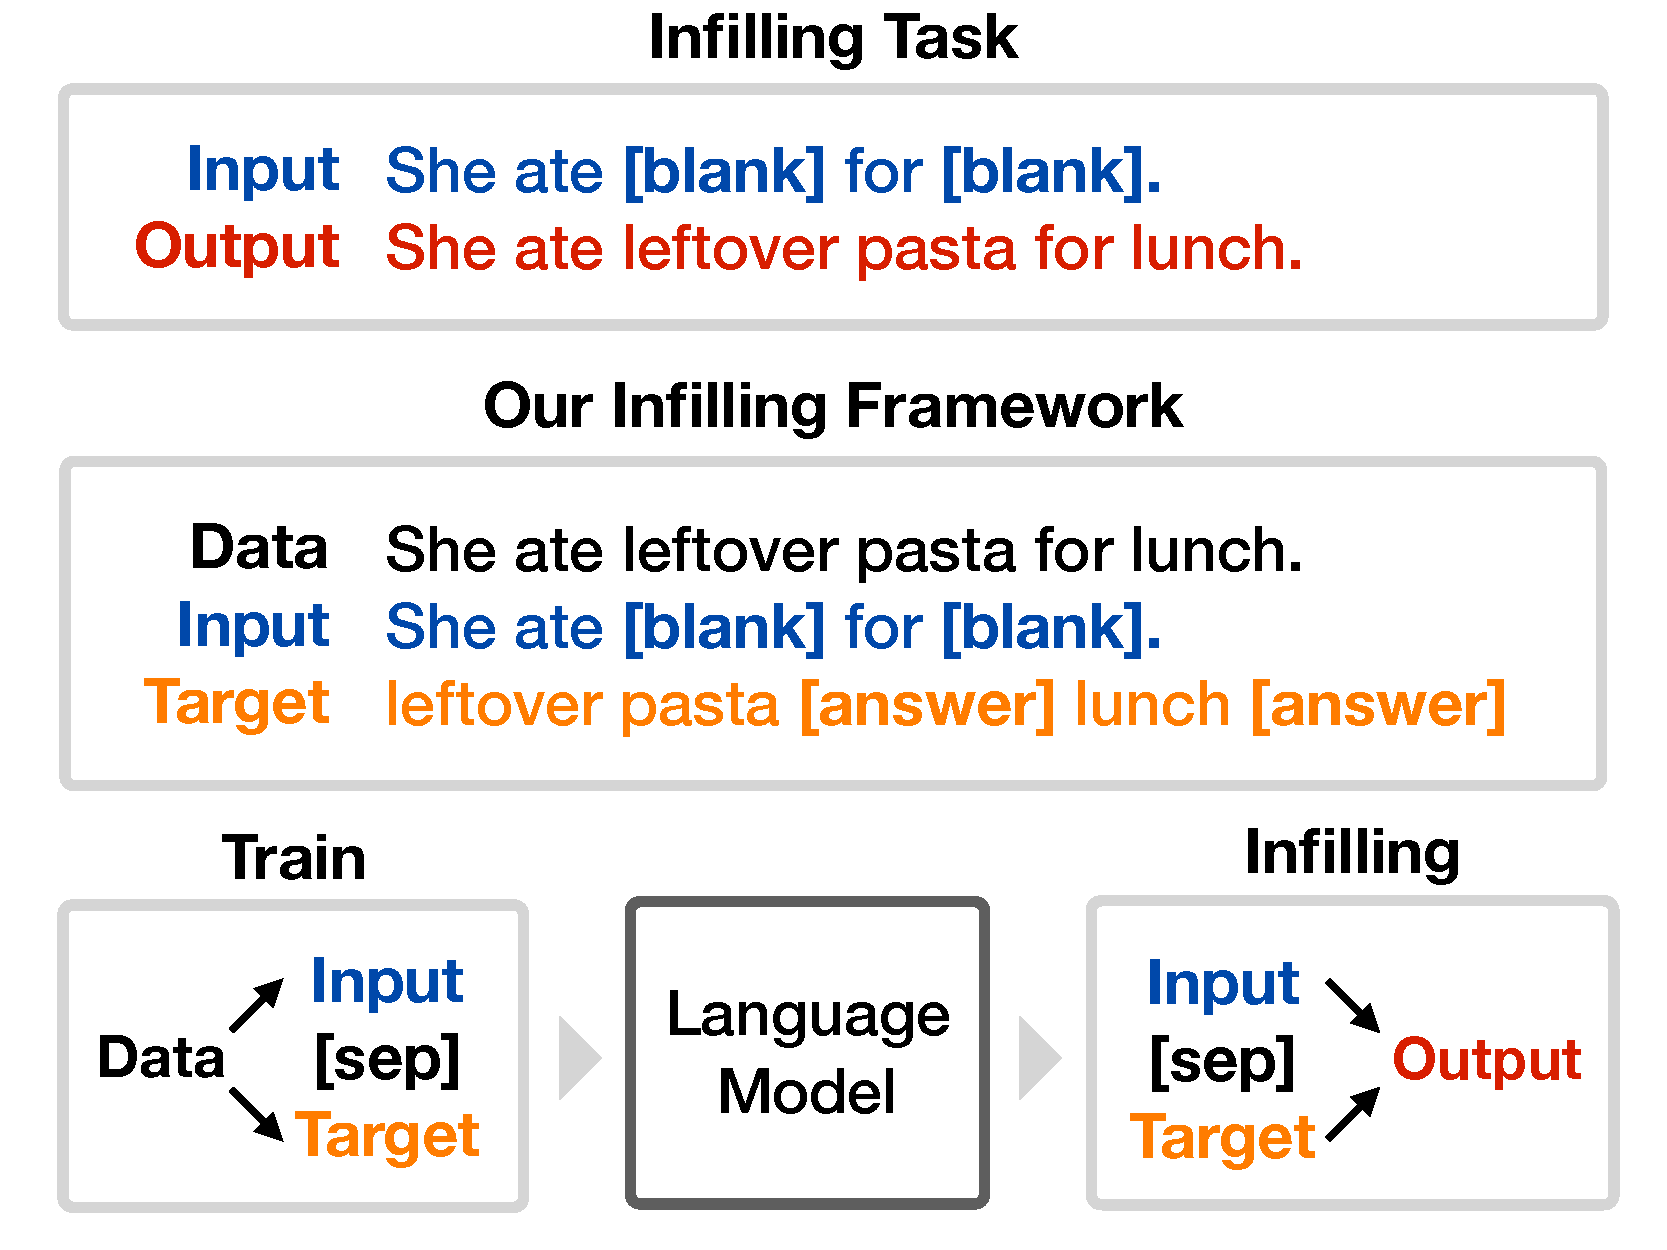
\includegraphics[width=1\linewidth]{acl2020-templates/figures/ilm_figure1_final.pdf}
    \caption{
    %Overview of our infilling framework.
    We consider the task of infilling, which takes incomplete text as input and outputs completed text.
    To tackle this task, our framework constructs training examples by masking random spans to generate pairs of inputs (text with blanks) and targets (answers for each blank). 
    We then train unidirectional language models on the concatenation of each pair.
    Once trained, a model takes text input with blanks, predicts the answers, and then combines them to produce the output.
    }
    \label{fig:infilling_training_example}
    \vspace{-5mm}
\end{figure}

Text infilling is the task of predicting missing spans of text which are consistent with the preceding and subsequent text.\footnote{Text infilling is a generalization of the \emph{cloze} task~\citep{taylor1953cloze}---cloze historically refers to infilling individual words.} 
Systems capable of infilling have the potential to enable rich applications such as assisting humans in
editing or revising text~\citep{shih2019xl}, 
connecting fragmented ideas~\citep{ai2019haim}, 
and restoring ancient documents~\citep{assael2019restoring}. 
Rather than targeting a particular application, our goal here is to provide a general, flexible, and simple infilling framework which can convincingly infill in a variety of domains.

A special case of infilling is language modeling: 
predicting text given preceding but not subsequent text.\footnote{In this paper, language modeling always refers to ordinary LMs, i.e., ``unidirectional,'' ``autoregressive,'' or ``left-to-right.''}
Language models are 
(1)~capable of generating remarkably coherent text~\citep{zellers2019defending,see2019massively},
(2)~efficient at generating text, 
and 
(3)~conceptually simple, 
but cannot infill effectively as they can only leverage context in a single direction (usually the past).
On the other hand, 
strategies such as BERT~\citep{devlin2019bert} and SpanBERT~\citep{joshi2019spanbert} are able to infill using both preceding and subsequent text. 
However, their use of bidirectional attention limits their infilling capabilities to fixed-length spans. 
This is problematic as---for many applications---we may not know the length of a missing span \emph{a~priori}. 
\citet{zhu2019text} propose a method capable of infilling variable-length spans, but it uses a specialized architecture and hence cannot easily leverage large-scale pre-trained models.

In this work, 
we present infilling by language modeling (ILM), 
a simple framework which enables LMs to infill variable-length spans while preserving their aforementioned benefits:
generation quality, efficient sampling, and conceptual simplicity. 
Our framework involves a straightforward formulation of the infilling task which, as we demonstrate, can be learned effectively by existing LM architectures. 
As shown in \Cref{fig:infilling_training_example},
our approach concatenates artificially-masked text with the text which was masked, and adopts a standard LM training (or fine-tuning) procedure on such examples. 
Once trained, infilling can be performed for a document with blanks by using the LM to generate text and then replacing the blanks with this text.

In addition to its conceptual simplicity, 
our experiments show that ILM enables off-the-shelf LMs to infill effectively. 
Furthermore, we find that infilling performance improves when starting from a large-scale pre-trained LM (as opposed to training from scratch), 
suggesting an additional benefit of using our model-agnostic framework compared to approaches which require specialized architectures.

We provide an interactive web demo of models trained under our framework. 
This demo can infill multiple variable-length spans with different granularities (e.g. words, n-grams, and sentences) on the domains of short stories, scientific abstracts, and song lyrics: 
\url{https://chrisdonahue.com/ilm}.
All code, data, and trained models are available at 
\url{https://github.com/chrisdonahue/ilm} and also on the CodaLab platform at  \url{https://worksheets.codalab.org/worksheets/0x9987b5d9cce74cf4b2a5f84b54ee447b}.